\documentclass{beamer}

\usepackage[utf8]{inputenc} % Language and font encoding
\usepackage[icelandic]{babel}
\usepackage[T1]{fontenc}


\usepackage{tikz}
\usepackage[listings,theorems]{tcolorbox}
\usepackage{booktabs}
\usepackage{minted} %Minted and configuration
\usemintedstyle{default}

\renewcommand{\theFancyVerbLine}{\sffamily \arabic{FancyVerbLine}}
%%%%%%%%%%%
% More math
%%%%%%%%%%%
\newcommand{\Mod}[1]{\ \text{mod}\ #1}

%%%%%%%%%%%%%%%%%%%%%%
% Beamer configuration
%%%%%%%%%%%%%%%%%%%%%%
\setbeamertemplate{navigation symbols}{}
\usecolortheme{dove}
\setbeamercolor{frametitle}{fg=white}

\usebackgroundtemplate%
{%
\vbox to \paperheight{

\includegraphics[width=\paperwidth]{Pics/hi-slide-head-2016}

\vfill
\hspace{0.5cm}
\includegraphics[width=0.3\paperwidth]{Pics/hi-von-logo}
\vspace{0.4cm}
    }%
}

\AtBeginSection[]
{
  \begin{frame}<beamer>
    \frametitle{Yfirlit}
    \tableofcontents[currentsection]
  \end{frame}
}

\setbeamerfont{frametitle}{size=\normalsize}
\addtobeamertemplate{frametitle}{}{\vspace*{0.5cm}}

%%%%%%%%%%%%%%%%%%%%%%%%%
% tcolorbox configuration
%%%%%%%%%%%%%%%%%%%%%%%%%

% Setup from: http://tex.stackexchange.com/a/43329/21638
\tcbset{%
    noparskip,
    colback=gray!10, %background color of the box
    colframe=gray!40, %color of frame and title background
    coltext=black, %color of body text
    coltitle=black, %color of title text 
    fonttitle=\bfseries,
    alerted/.style={coltitle=red, colframe=gray!40},
    example/.style={coltitle=black, colframe=green!20, colback=green!5},
}


%%%%%%%%%%%%%%%%%%%%%%%
% Further configuration
%%%%%%%%%%%%%%%%%%%%%%%
\hypersetup{colorlinks=true,pdfauthor={Eirikur Ernir Thorsteinsson},linkcolor=blue,urlcolor=blue}
\graphicspath{{./Pics/}}

\author{Eiríkur Ernir Þorsteinsson}
\institute{Háskóli Íslands}
\date{Haust 2016}

\title{Tölvunarfræði 1a}
\subtitle{Vika 5, fyrri fyrirlestur}

\begin{document}

\begin{frame}
\titlepage
\end{frame}

\section{Inngangur}

\begin{frame}{Í síðasta þætti\ldots}
\begin{itemize}
 \item Föll
 \item \texttt{if}
 \begin{itemize}
  \item \texttt{if-else}
  \item Hreiðruð \texttt{if}
 \end{itemize}
 \item \texttt{switch}
 \item \texttt{is}-föll
\end{itemize}
Kaflar: 4.3, 4.4, 4.6
\end{frame}

\begin{frame}[fragile]{Gömul fyrirlestraæfing}
Skrifið ykkar eigin útgáfu af \texttt{isrow} fallinu. \pause
\begin{minted}[frame=lines]{matlab}
function isARow = myIsRow(matrix)
% Skilar sönnu ef tvívíða fylkið matrix er 
% með nákvæmlega eina línu
    dimensions = size(matrix);
    if dimensions(1) == 1
        isARow = true;
    else
        isARow = false;
    end
end
\end{minted}

\end{frame}

\begin{frame}{Hugtakið ``lykkja''}
\begin{itemize}
 \item Hingað til hefur hver skipun verið framkvæmd nákvæmlega einu sinni
 \item Við getum látið Matlab endurtaka framkvæmd skipunar, oftast með smávægilegum breytingum, með því að nota lykkju (e. \emph{loop})
 \begin{itemize}
  \item Hægt væri að einfaldlega skrifa skipunina oft, en það verður nær ómögulegt þegar ``oft'' verður að ``mjög oft''
 \end{itemize}
 \item Flest forritunarmál hafa lykkjuskipanir
 \begin{itemize}
  \item \emph{Mjög} mikið notaðar í öðrum forritunarmálum
 \end{itemize}
 \item í Matlab er oft hægt að komast hjá því að nota lykkjur með því að nýta getu Matlab til að vinna með vigra og fylki
 \item Að keyra lykkjur er kallað að \textbf{ítra} (e. \emph{iterate})
\end{itemize}
\end{frame}

\begin{frame}{Tvær gerðir lykkja}
\begin{itemize}
 \item Talningalykkjur (e. \emph{counting loops})\footnote{Viðfangsefni okkar í dag}
 \begin{itemize}
  \item Skipanir endurteknar ákveðið mörgum sinnum
  \item Notaðar þegar fjöldi endurtekninga er þekktur fyrirfram
 \end{itemize}
 Dæmi: \emph{Prentaðu ``hæ'' 10 sinnum.}
 \pause
 \item Skilyrtar lykkjur (e. \emph{conditional loops})
 \begin{itemize}
  \item Skipanir endurteknar á meðan ákveðið skilyrði er satt
  \item Notaðar þegar fjöldi endurtekninga er ekki þekktur fyrirfram
 \end{itemize}
 Dæmi: \emph{Prentaðu ``hæ'' þar til notandinn skrifar ``hættu''.}
\end{itemize}
\end{frame}

\section{For-lykkjur í Matlab (5.1)}

\begin{frame}[fragile]{for-lykkjur}
\begin{itemize}
 \item Almennt form for-lykkja:
\begin{verbatim}
for breyta = svið
  skipanir
end
\end{verbatim}
 \item \emph{Svið}ið er vigur. 
 \begin{itemize}
  \item Breytan fær hvert gildi sviðsins á fætur öðru og skipanirnar eru framkvæmdar fyrir öll gildin
  \item Fyrst fær hún fyrsta gildi vigursins, svo annað\ldots
  \item Allar skipanir inni í lykkjunni eru framkvæmdar einu sinni fyrir hvert gildi sviðsins
 \end{itemize}
\end{itemize}
\end{frame}

\begin{frame}{Dæmi um for-lykkju}
\begin{columns}
\column{0.5\textwidth}
Skráin \texttt{forExample.m}
\begin{center}
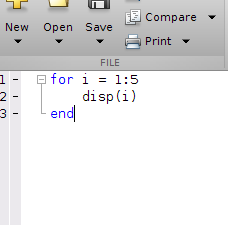
\includegraphics[width=0.8\linewidth]{Pics/for-example}
\end{center}
\column{0.5\textwidth}
Keyrsla í skipanaglugga
\begin{center}
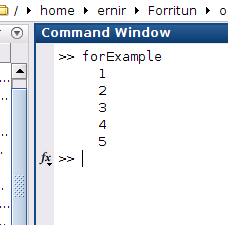
\includegraphics[width=0.8\linewidth]{Pics/for-example-run}
\end{center}
\end{columns}
\end{frame}

\begin{frame}[fragile]{Mismunandi for-lykkjur}
Getum haft hvaða vigur sem er í haus for-lykkjunnar
\begin{columns}
\column{0.5\textwidth}
Lykkjan
\begin{minted}[frame=lines]{matlab}
for i = 0:5:15
    disp(i)
end
\end{minted}
skrifar
\begin{verbatim}
0
5
10
15
\end{verbatim}


\column{0.5\textwidth}
Lykkjan 
\begin{minted}[frame=lines]{matlab}
for letter = 'abc'
    disp(letter)
end
\end{minted}
skrifar
\begin{verbatim}
a
b
c
\end{verbatim}
Strengir eru vigrar af bókstöfum.
\end{columns}
\end{frame}

\begin{frame}[fragile]{Ítrunarbreyta}
\begin{itemize}
 \item Oftast notum við ítrunarbreytuna í hverri ítrun lykkjunnar
 \begin{itemize}
  \item Því má þó sleppa
  \item Þá er lykkjan einungis notuð til að ákveða hversu oft eitthvað á að gerast
  \item Lykkjan keyrð jafn oft og vigurinn er langur
 \end{itemize}
\end{itemize}
\end{frame}

\begin{frame}[fragile]{Ítrunarbreyta}
\begin{columns}
\column{0.65\textwidth}
\begin{minted}[frame=lines]{matlab}
% Þessi skipanaskrá biður notanda 
% þrisvar um tölu og skrifar hana út

for i = 1:3
    n = input('Tölu takk: ');
    fprintf('%.1f slegið inn\n', n);
end
\end{minted}
\column{0.35\textwidth}
\begin{verbatim}
>> forEcho
Tölu takk: 3
3.0 slegið inn
Tölu takk: 1
1.0 slegið inn
Tölu takk: 5
5.0 slegið inn
>>
\end{verbatim}
\end{columns}
\vspace{\baselineskip}
Hér er ítrunarbreytan \texttt{i} ekki notuð.
\end{frame}

\begin{frame}[fragile]{Útreikningar}
\begin{itemize}
 \item Lykkjur eru gjarnan notaðar til að framkvæma útreikninga
 \item Dæmi: Reikna upp úr summunni $1 + 2 + \ldots + n$
\end{itemize}

\begin{minted}[frame=lines]{matlab}
vSum = 0;
for i = 1:n
    vSum = vSum + i;
end
\end{minted}

(Þennan kóða væri upplagt að setja í fall sem tekur inn \texttt{n} og skilar \texttt{vSum})

\end{frame}

\begin{frame}{Fyrirlestraæfing}
Skráið ykkur inn á \url{http://socrative.com/} og gerið fyrstu tvær spurningarnar

Herbergisnúmer = \texttt{TOL105G2016}

Notendanafn = HÍ-tölvupóstfang

Lagið:


\emph{\small 99 bottles of beer on the wall, 99 bottles of beer.

Take one down and pass it around, 98 bottles of beer on the wall.

98 bottles of beer on the wall, 98 bottles of beer.

Take one down and pass it around, 97 bottles of beer on the wall.}
\end{frame}

\subsection{Forúthlutun í lykkju}

\begin{frame}{Forúthlutun vigra}
\vspace{\baselineskip}
\begin{itemize}
 \item Algengt er að í hverri ítrun lykkju bætist við nýjar upplýsingar sem þarf að geyma
 \begin{itemize}
  \item Niðurstöður útreikninga
  \item Innsláttur frá notanda
 \end{itemize}
 \item Í Matlab er upplýsingunum þá bætt við vigur, en til þess eru tvær leiðir
 \begin{itemize}
  \item Byrja með tóman vigur og bæta nýja gildinu við hann
  \begin{itemize}
   \item Vigurinn er þá alltaf að stækka - en það að stækka vigur er dýr (tímafrek) aðgerð í Matlab
  \end{itemize}
  \item Forúthluta (e. \emph{preallocate}) vigri af réttri stærð og setja síðan hverja innslegna tölu í rétt sæti
  \begin{itemize}
   \item Algengt bragð í Matlab
  \end{itemize}
 \end{itemize}
\end{itemize}
\end{frame}

\begin{frame}[fragile]{Dæmi: Innsleginn vigur}
Sett í skrána \texttt{longerVector.m}:
\begin{minted}[frame=lines]{matlab}
% Skipanaskrá sem býr til vigur úr innslegnum tölum
% Skipanaskrá sem býr til vigur úr innslegnum tölum
n = 3;
storage = []; % Vigurinn storage byrjar tómur
for i = 1:n
  newNum = input('Sláðu inn tölu til geymslu: ');
  storage = [storage newNum]; % bætt við aftast í storage
end
\end{minted}
\end{frame}

\begin{frame}[fragile]{Keyrsla longerVector}
\begin{columns}
\column{0.5\textwidth}
\begin{verbatim}
>> longerVector
Sláðu inn tölu til geymslu: 3
Sláðu inn tölu til geymslu: 6
Sláðu inn tölu til geymslu: 7
>> storage
storage =
   3   6   7
\end{verbatim}
\column{0.5\textwidth}
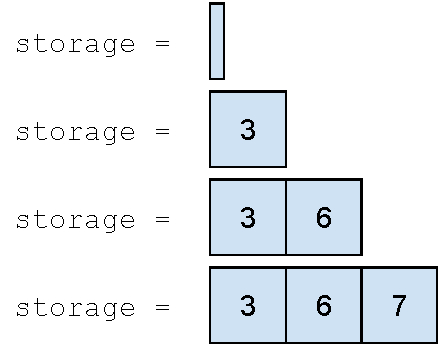
\includegraphics[width=\linewidth]{Pics/vector-expansion}

Sífellt stærra minnissvæði þarf til að geyma vigurinn.
\end{columns}
\end{frame}

\begin{frame}{Stækkun vigurs}
\begin{itemize}
 \item Hvers vegna er svo dýrt að stækka vigur?
\begin{itemize}
 \item Ef vigur er 10 stök og við viljum bæta einu staki við hann þá er ekki endilega hægt að nota til þess minnishólfið sem er fyrir aftan vigurinn
 \item Þá þarf að taka frá svæði á öðrum stað í minninu fyrir 11 stök, afrita stökin 10 af gamla staðnum og setja síðan 11-ta stakið í síðasta sætið
 \item Loks er 10-hólfa minnisplássinu skilað aftur, svo hægt sé að endurnota það
\end{itemize}
 \item Töluvert umstang!
\end{itemize}
\end{frame}

\begin{frame}[fragile]{Forúthlutun}
Getum gert betur:
\begin{minted}[frame=lines]{matlab}
% Skipanaskrá sem býr til vigur úr innslegnum tölum
n = 3;
storage = zeros(1,n); % storage byrjar í lengd n
for i = 1:n
  newNum = input('Sláðu inn tölu til geymslu: ');
  storage(i) = newNum; % newNum sett í sæti i
end
\end{minted}
\end{frame}

\begin{frame}[fragile]{Keyrsla longerVector}
\begin{columns}
\column{0.5\textwidth}
\begin{verbatim}
>> preallocatedVector
Sláðu inn tölu til geymslu: 3
Sláðu inn tölu til geymslu: 6
Sláðu inn tölu til geymslu: 7
>> storage
storage =
   3   6   7
\end{verbatim}
\column{0.5\textwidth}
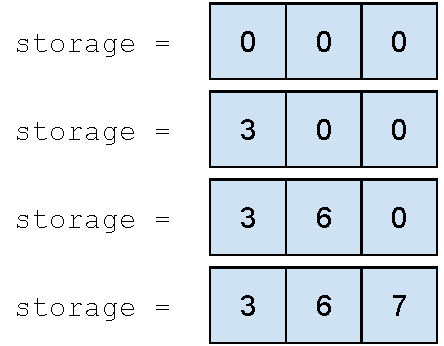
\includegraphics[width=\linewidth]{Pics/no-vector-expansion}

Stærð minnissvæðisins breytist ekki, bara innihaldið.
\end{columns}
\end{frame}

\subsection{if í for}

\begin{frame}[fragile]{if-setning í for-lykkju}
\vspace{\baselineskip}
\begin{itemize}
 \item Hægt er að nota \texttt{if} inni í \texttt{for}
 \begin{itemize}
  \item T.d. til þess að vinna bara með sum stök vigursins
 \end{itemize}
\end{itemize}

\begin{minted}[frame=lines]{matlab}
vSum = 0;
for i = 1:length(v)
    if v(i) >= 0
       vSum = vSum + v(i);
    end
end
\end{minted}
\begin{itemize}
 \item Hér eru öll jákvæð stök vigursins lögð saman.
\end{itemize}
\end{frame}

\begin{frame}[fragile]{Dæmi um reiknirit}
\vspace{\baselineskip}
\begin{minted}[frame=single]{matlab}
function outMin = myMinVec(vec)
% myMinVec skilar minnsta gildi vigurs
% Notkun:  myMinVec(vigur)
 
   outMin = vec(1); % Upphafsstillt með fyrsta staki
   for i = 2:length(vec)
      if vec(i) < outMin
         outMin = vec(i); % Ef minna, þá minnst
      end
   end % Öll stökin hafa verið athuguð
end
\end{minted}
\end{frame}

\subsection{Hreiðraðar for-lykkjur (5.2)}

\begin{frame}[fragile]{Hreiðraðar for-lykkur}
\begin{itemize}
 \item Hvaða skipanir sem er geta verið inni í lykkju
 \item Hægt er að setja lykkju inn í lykkju!
 \begin{itemize}
  \item Þá framkvæmist innri lykkjan öll fyrir hverja ítrun af ytri lykkjunni
  \item Mjög algengt þegar unnið er með fylki
  \begin{itemize}
   \item Fyrir allar línur í fylkinu, gera eitthvað fyrir alla dálka í þeirri línu
  \end{itemize}
 \end{itemize}
\end{itemize}
\end{frame}

\begin{frame}[fragile]{Dæmi: Skrifa út kassa af stjörnum}
\begin{columns}
\column{0.6\textwidth}
Skipanaskráin \texttt{starBox.m}, skrifar út $3 \times 5$ kassa af stjörnum.
\begin{minted}[frame=lines]{matlab}
% Prentar út kassa af stjörnum
for r = 1:3
    for c = 1:5
        fprintf('*');
    end
    fprintf('\n');
end
\end{minted}
\column{0.4\textwidth}
\begin{verbatim}
>> starBox
*****
*****
*****
\end{verbatim}
\end{columns}
\end{frame}

\begin{frame}[fragile]{Dæmi: Margföldunartafla (bls. 158)}
\begin{columns}
\column{0.7\textwidth}
\begin{minted}[frame=lines]{matlab}
function outmat = multtable(rows, columns)
% multtable returns a multiplication table
% Format: multtable(nRows, nColumns)

   outmat = zeros(rows,columns);
   for i = 1:rows
      for j = 1:columns
        outmat(i,j) = i * j;
      end
   end
end
\end{minted}
\column{0.30\textwidth}
\begin{verbatim}
>> multtable(3,3)
ans =

   1   2   3
   2   4   6
   3   6   9
\end{verbatim}
\end{columns}
\end{frame}

\begin{frame}[fragile]{Margföldunartafla (bls. 159)}
\vspace{\baselineskip}
Getum notað fallið í skipanaskrá (hér \texttt{createmulttab.m})
\begin{minted}[frame=lines]{matlab}
% Prompt the user for rows and columns and
%  create a multiplication table to store in
%  a file "mymulttable.dat"
 
num_rows = input('Enter the number of rows: ');
num_cols = input('Enter the number of columns: ');
multmatrix = multtable(num_rows, num_cols);
save mymulttable.dat multmatrix -ascii
\end{minted}
\end{frame}

\begin{frame}[fragile]{Fyrirlestraæfing}
Skráið ykkur inn á \url{http://socrative.com/} og klárið spurningarnar.

Herbergisnúmer = \texttt{TOL105G2016}

Notendanafn = HÍ-tölvupóstfang
\end{frame}



\end{document}
